%
% File: chap01.tex
% Author: Victor F. Brena-Medina
% Description: Introduction chapter where the biology goes.
%
\let\textcircled=\pgftextcircled
\chapter{Active Brownian Spheres in Random and Porous Environments}
\label{chap:confinement}


\initial{W}hen the transport of active particles (both biological microswimmers and synthetic particles) occurs in complex environments, the resultant dynamics depend on an emergent the interplay between the mobility of the active component and the quenched disorder of the environment. 
Here we explore structural and dynamical properties of Active Brownian Particles (ABP) in random environments composed of fixed obstacles in three dimensions. We consider different degrees of spatial correlation of the obstacles, by pinning particles either in (non-overlapping) random positions or in a percolating gel-like structure, and provide an extensive characterisation of the structure and dynamics of ABP in complex environments. We find that the confinement increases the heterogeneity of the dynamics, with new populations of absorbed and localised particles appearing close to the obstacles. This heterogeneity has a profound impact on the motility induced phase separation (MIPS) exhibited by the particles at high activity, ranging from a standard growth in random disorder, to a bicontinuous phase separation in porous environments.


\section{Introduction}
%\label{section:intro}
Active Matter concerns systems comprised of individual bodies undergoing motion via self-propulsion \cite{ramaswamy2017}. This description encompasses a plethora of systems over a wide range of lengthscales from biological microswimmers \cite{elgeti2015}, schools of fish \cite{yang2022}, bird flocks \cite{cavagna2014}, to human crowds \cite{koyama2020}. 
While these systems can all be classified as active matter, accurate models must be tailored to the specifics of each system and its environment. For active matter on mesoscopic lengthscales (nm to $\mu$m), the most common systems are bacteria \cite{zhang2010b,lopez2015,jepson2013} and self-propelling colloids \cite{buttinoni2013,bricard2013,mauleonamieva2020}, the dynamics of which can be described by run and tumble dynamics and active Brownian motion respectively. These models (which are equivalent over long time-scales \cite{cates2013}) have been studied extensively and can faithfully reproduce the unique dynamical phenomena of these out-of-equilibrium systems such as motility-induced phase separation \cite{cates2015,marchetti2016}. 


If we are to apply these models to a biological context, it is essential that we study the dynamics of active particles in environments that are relevant to their real-world counterparts. For biological active matter on mesoscopic lengthscales this means environments like porous soils \cite{gannon1991} and organic tissues \cite{isermann2017}. Environments such as these have several qualities in common, they are often crowded, random and irregular. This of course has an impact on the transport or displacement of the active bodies inside these spaces \cite{bechinger2016a}. 

In equilibrium systems, the dynamics of fluids in dense and complex environments has long been an area of interest. For example, the inclusion of specific structures into dense fluids has proven significant for advancements towards understanding the glass transition and on supercooled liquids \cite{alcoutlabi2005,kim2011}. Furthermore, the addition of randomly pinned particles within a dense ensemble is known to greatly slow the dynamics of such systems, providing access to distant states \cite{russo2010,karmakar2013,kim2011,ozawa2015}. A special kind of localisation has been explored in glass-forming systems \cite{biroli2008}, and which may be realised (so far in two dimensions) using colloidal systems \cite{gokhale2016,gokhale2014a,williams2018}.
. Here \textit{pinning} i.e. immobilising a fraction of the particles, provides access to the so-called ideal glass, a putative amorphous state of very low configurational entropy whose diverging timescales render it otherwise inaccessible to experiment or computer simulation \cite{berthier2011}.

For active systems, in the simplest case of a confining wall, a self-propelling sphere will accumulate at a wall as a consequence of the timescale of its persistent motion, even in the absence of hydrodynamic interactions \cite{elgeti2013}. For many-body systems in two-dimensions, the influence of disordered landscapes on to the dynamics of active systems has been shown to manifest in clogging and localisation transitions \cite{reichhardt2017,reichhardt2018,chepizhko2019a}, subdiffusion over long timescales \cite{chepizhko2013,zeitz2017,morin2017}, destruction of flocking clusters \cite{morin2017}, destruction of MIPS and the prevention of uniform wetting at boundaries \cite{dor2021}.
 Furthermore, manipulation of complex environments has been shown to provide a degree of control over the transport of active matter in the form of sorting \cite{volpe2011a}, and control over net flow directions \cite{borba2020}.


In three-dimensions, active Brownian particles (ABP) exhibit rich phase behaviour such as MIPS \cite{wysocki2014,stenhammar2014}, and the formation of active crystals \cite{omar2021a,moore2021a}. However, the question of how ABP couple to a complex surrounding environment remains unanswered. To date, there have been few experiments observing three-dimensional mesoscale active matter. In one study a random heterogeneous environment was found to impose strong inhibitions on active transport of bacteria \cite{bhattacharjee2019}, and in another study the impact dimensionality was made clear, with the dominance of three-dimensional structure in the presence of an anisotropic potential \cite{sakai2020}. Due to the experimental challenge of realising active systems in 3D this is an under-developed area of the field. Insight into the transport of active matter in 3D complex environments could provide a major step towards control of such systems and aid advancements towards applications such as drug delivery.


In the present chapter, we perform three-dimensional molecular dynamics simulations of active Brownian particles in complex heterogeneous environments. To model such environments, we choose two example structures: a random array of pinned particles, providing an extension of disordered random obstacle studies to 3D; and a continuous, percolating porous network, simulating the complex environments typical to active matter under confinement. Furthermore, we will investigate the structural and dynamical properties of ABP within these structures, with a focus on phase separation and how this varies from MIPS in bulk suspensions.
 
The chapter is organised as follows: in Section \ref{section:methods} we outline the computational methods used to study these systems, in section \ref{section:results} we discuss the results of the simulations, and finally in section \ref{section:conclusion} we summarise and conclude our findings and discuss future work in this area. 

\section{Model and methods}
\label{section:methods}

\subsection{Active particles}

We model active bodies as active Brownian particles, which propel with a constant velocity $v_p$ along their individual direction vectors $\boldsymbol{e}$, which in turn are subject to rotational diffusion. 
We implement this model through molecular dynamics simulations using a customised version of the open source LAMMPS package \cite{moore2021a}, which integrates the following
equations of motion:


\begin{equation}
    \dot{\mathbf{r}}=v_{p} \mathbf{e}+\beta D_{T}\mathbf{F} +\sqrt{2D_{T}}\boldsymbol{\xi_T}
    \label{eq:Eom1}
\end{equation}


\begin{equation}
    \dot{\mathbf{e}}=\sqrt{2D_{R}}\boldsymbol{\xi_R} \times \mathbf{e}
    \label{eq:Eom2}
\end{equation}


\noindent
Here $\dot{\mathbf{r}}$ is the particle velocity, $v_p$ is the magnitude of the constant active velocity, and $\boldsymbol{F}$ is the inter-particle force. The thermal fluctuations promoting translational diffusion are included in the Gaussian white-noise term
$\boldsymbol{\xi_T}$, where $\langle\boldsymbol{\xi_T}\rangle=0$, and $D_{T}$ is the translational diffusion coefficient. Thermal noise driving rotational diffusion of the direction vector $\boldsymbol{e}$ is represented by $\boldsymbol{\xi_R}$,  where $\langle\boldsymbol{\xi_R}\rangle=0$, and $D_{R}$ is rotational diffusion coefficient. The two diffusion coefficients are related via $D_{T} = D_{R}\sigma^{2}/3$, where $\sigma$ is the particle diameter. Time is scaled in units of the characteristic rotational diffusion time $\tau_R = 1 / (2D_R)$ \cite{wysocki2014}. 

%For all simulations in this work $\beta = 5$, $m=1$, $\sigma=1$. 

The active particles are modelled as being similar to hard spheres and to achieve this we include a Weeks-Chander-Andersen (WCA) inter-particle potential, which takes the form:


\begin{equation}
\beta u(r_{ij}) = \begin{cases}
4 \beta \varepsilon\left[\left(\frac{\sigma}{r_{ij}}\right)^{12} - \left(\frac{\sigma}{r_{ij}}\right)^{6}\right] + \varepsilon & r_{ij} \leq 2^{\frac{1}{6}}\sigma \\%&\text{se $\omega\in A$}\\
0 & r_{ij} > 2^{\frac{1}{6}}\sigma   
\end{cases}
\label{eq:WCA}
\end{equation}


\noindent
where $\varepsilon$ is the interaction energy, $r_{ij}$ is the inter-particle distance, and $\beta=1/k_BT$ the thermal energy. 


Since we use the WCA interaction,
we cannot assume the hard particle diameter $\sigma$ to define a volume fraction. Furthermore, methods that determine an effective particle diameter such as Barker--Henderson effective hard sphere diameter \cite{barker1967}, may not hold outside of equilibrium systems. Therefore, as in ref. \cite{martin-roca2021}, we use the total density $\rho = N / V$, where $N$ is the number of particles and $V$ is the volume of the system.  
We use the P\'{e}clet number to refer to the relative strength of the activity in the system, which we define as: $\pecl = v_p/\sigma D_{R}$. Throughout this work we keep $D_R$ constant, and vary $\pecl$ by changing the propulsion velocity $v_p$. 
Simulations are performed with periodic boundary conditions. The majority of the work is carried out in a cubic box of dimension length $L = 55\sigma$, with a total number of $N = 144000$ particles. In some cases, there was a need to sample from many state points and for these a smaller system was used where $L = 27.5\sigma$ and $N$ ranges from 18000 to 24000. Analysis at constant density is always conducted at $\rho = 0.87$. This state point is chosen such that it lies below the freezing line in the bulk.
 

\subsection{Complex environments}
The complex environments relevant to microscopic biological systems are often irregular and random in nature. To investigate the dynamical properties of ABP under these conditions, one must prepare obstacle geometries that satisfy these requirements. Here we consider two primary structures; porous networks and randomly pinned particles. In addition to this, we include simulations studying the bulk dynamics of ABPs as a reference, these bulk simulations use the approach outlined in the previous section.

\begin{figure*}
	\centering
	\includegraphics[width=\linewidth]{chapters/activeConfinement/figsActiveConfinement/figObstacles.png}
	\caption[Confining structures: colloidal gels and random pinning]{\textbf{a} Percolating gel network at density $\rho= 0.38$. \textbf{b} Cross-section through the gel network of depth 2$\sigma$.  \textbf{c} A collection of randomly pinned obstacles at $\rho =0.31$. \textbf{d} Cross-section through the random obstacles of depth 2$\sigma$. \textbf{e-f} Gel network (grey) filled with active particles (blue) to a total density $\rho=0.42$. \textbf{g-h} Random obstacles filled with active particles to a total density $\rho=0.42$.}
	\label{fig:Gel_vs_Rand}
\end{figure*}

In the following section, the methodology through which the two complex environments are created and characterised is outlined. A schematic depicting these two environment structures is displayed in Fig. \ref{fig:Gel_vs_Rand}, featuring 3D renderings of each environment type, along with a cross-sectional slice. The porous network (Fig. \ref{fig:Gel_vs_Rand}a-b), is a heterogeneous system, comprised of two distinct meso-phases which percolate through the entire simulation space, comprised of the particle–rich phase and a particle–poor phase in which for our parameters no particles are found.  The random environment (Fig. \ref{fig:Gel_vs_Rand}c-d), is comprised of randomly pinned particles that create number of discrete obstacles dispersed throughout the system. 


\textit{Preparation of the gel ---}
In this work the porous network is modelled as a colloidal gel, specifically a colloid-polymer mixture \cite{poon2002}. When colloids (which can be thought of as hard-spheres) are suspended at a suitable density, and in the presence of sufficient non-adsorbing polymer, the system begins to phase separate via spinodal decomposition which is then arrested, often leaving a bicontinuous network \cite{zaccarelli2007,royall2021}.  
This phase separation is a result of depletion inte ractions \cite{lekkerkerker2011}, which are entropy driven interactions that manifest in the assembly of colloids such that the depletants (polymers) have the greatest free volume.
The (effective) depletion interaction between the particles is modelled with a short-range attractive potential \cite{royall2008},  in this work the Morse potential is used:
\begin{equation}                                                                                                                                                                                                                                                                                                                                                                                                                                                                                                                                                                                                                                                                                                                                                                                                                                                                                                                                                                                                                                                                                                                                                                                                                                                                                                                                                                                                                                                                                                                                                                                                                                                                                                                                                                                                                                                                                                                                                                                                                                                                                                                                                                                                                                                                                                                                                                                                                                                                                                                                                                                                                                                                                                                                                                                                                                                                                                                                                                                                                                                                                                                                                                                                                                                                                                                                                                                                                                                                                                                                                                                                                                                                                                                                                                                                                                                                                                                                                                                                                                                                                                                                                                                                                                                                                                                                                                                                                                                                                                                                                                                                                                                                                                                                                                                                                                                                                                                                                                                                                                                                                                                                                                                                                                                                                                                                                                                                                                                                                                                                                                                                                                                                                                                                                                                                                                                                                                                                                                                                                                                                                                                                                                                                                                                                                                                                                                                                                                                                                                                                                                                                                                                                                                                                                                                                                                                                                                                                                                                                                                                                                                                                                                                                                                                                                                                                                                                                                                                                                                                                                                                                                                                                                                                                                                                                                                                                                                                                                                                                                                                                                                                                                                                                                                                                                                                                                                                                                                                                                                                                                                                                                                                                                                                                                                                                                                                                                                                                                                                                                                                                                                                                                                                                                                                                                                                                                                                                                                                                                                                                                                                                                                                                                                                                                                                                                                                                                                                                                                                                                                                                                                                                                                                                                                                                                                                                                                                                                                                                                                                                                                                                                                                                                                                                                                                                                                                                                                                                                                                                                                                                                                                                                                                                                                                                                                                                                                                                                                                                                                                                                                                                                                                                                                                                                                                                                                                                                                                                                                                                                                                                                                                                                                                                                                                                                                                                                                                                                                                                                                                                                                                                                                                                                                                                                                                                                                                                                                                                                                                                                                                                                                                                                                                                                                                                                                                                                                                                                                                                                                                                                                                                                                                                                                                                                                                                                                                                                                                                                                                                                                                                                                                                                                                                                                                                                                                                                                                                                                                                                                                                                                                                                                                                                                                                                                                                                                                                                                                                                                                                                                                                                                                                                                                                                                                                                                                                                                                                                                                                                             \beta u\left(r_{ij}\right)=\beta \varepsilon \exp \left[a_{0}\left(\sigma-r_{ij}\right)\right]\left(\exp \left[a_{0}\left(\sigma-r_{ij}\right)\right]-2\right)
    \label{eq:Morse}
\end{equation}


\noindent
where $a_0=33$ is a range parameter. 

To create the gel structures in simulation, we begin with particles in a simple cubic crystal at the desired density, and then evolve this system according to Brownian dynamics (eq. (\ref{eq:Eom1}), for $v_p = 0$), with the particles interacting via the Morse potential Eq. (\ref{eq:Morse}). This system is then evolved for $5 \times 10^{7}$ integration steps, which is equivalent to 1200$\tau_B$. $\tau_B$ is the Brownian time $\tau_B=(\sigma /2)^2 / 6D_T$,  which defines the timescale of the relaxation of the particle velocity. As this system evolves, the branches of the network coarsen and the potential energy of the system drops. This happens rapidly at the beginning, and then much more slowly as the system approaches equilibrium. It is at this point that the gel is then \textit{frozen}, meaning that the gel particle coordinates are kept constant to form the solid porous network (Fig. \ref{fig:Gel_vs_Rand}a-b).

With the gel in place, the positions of the free particles are initialised via the Lubachevsky--Stillinger algorithm \cite{lubachevsky1990}. This method comprises the following steps: First, initial particle positions are randomly assigned. Then, the particles are slowly grown and displaced from an initial diameter $\sigma_{i}=0.1$, to the desired diameter $\sigma=1$, such that these particles experience minimal overlaps with themselves and with the frozen gel particles. Additionally, to guard against the presence of any small but sufficient remaining particle overlaps, a pre-run simulation with a soft potential is performed: 


\begin{equation}
u(r_{ij})=A\left[1+\cos \left(\frac{\pi r_{ij}}{r_{c}}\right)\right] \quad r_{ij}<r_{c}
\label{eq:soft}
\end{equation}


\noindent
where $r_c = 2^\frac{1}{6}$ is the potential cut-off, and the constant A is ramped from 0 to 100 over $1.2 \tau_R$ without activity. Following this the system is equilibrated again without activity, for particles following the equations of motion outlined in Eq. (\ref{eq:Eom1}) and Eq. (\ref{eq:Eom2}), and the WCA inter-particle potential Eq. (\ref{eq:WCA}). A low density example of this system is shown in Fig. \ref{fig:Gel_vs_Rand}e-f.


\textit{Random pinning ---}
For the randomly pinned configurations, a random configuration of particles is generated in the simulation box at the desired density. These particles then follow Brownian dynamics with the soft potential Eq. (\ref{eq:soft})  to eliminate any significant overlaps before the system is equilibrated with the WCA potential. Following this, a fraction of the particle ensemble is frozen creating the random obstacles. This fraction is chosen such that the volume accessible to the free particles is the same in both the gel network and the random pinning systems (Fig. \ref{fig:Gel_vs_Rand}c-d).
The fixing of the accessible free volume of the mobile particles enables comparison of observables in both environments. Fixing this is a necessary step as the difference in structure between the gel network and the random pins could result in the free particles operating at two different effective densities for the same number of frozen particles. 
For this, the density of the gel network is held constant and the number of pinned particles is varied as a function of the total density $\rho$. The total free volume available to the mobile particles is determined with the Voronoi volumes $V^i_{\textrm{voro}}$ for systems in the absence of activity. The sum of these volumes provides the total volume accessible to the free particles $\sum_{i}^N V^i_{\textrm{voro}}$, which are then averaged over ten independent simulation runs. This information is used to determine the fraction of particles to be pinned, such that $\sum_{i}^N V^i_{\textrm{\textrm{voro}}}$ for the free particles in the pinned system matches that of the porous network at the same density.  


\textit{Lengthscales in the complex environments ---} The interplay between the lengthscale of the two environments and the persistent motion of the active particles will have a large impact on the dynamics. Therefore, to characterise the lengthscale the obstacles impose on the active particles we will use the pore \textit{chord length}. The chord length is a measure of the distance between two interfaces in a homogeneous phase of a heterogeneous system. The pore chord length distribution can be defined as $p(\ell)$, it describes the probability of finding a chord inside the pores surrounding the network branches of a length $\ell$. We characterise the environments in this work by the mean pore chord length $<L_c>$. In practise, this is determined by measuring chords of varying lengths along each axis of the three dimensional sample that lie wholly within the pore phase \cite{whittle1999,testard2011}. The mean chord length was measured and averaged for six independent configurations for each environment species. The gel networks have a mean pore chord length $<L_c> = 6.62\sigma$, whereas for the random pinning system $<L_c> = 3.24\sigma$, almost half that of the gel system. 

%For the random pins, we can use the relation $(N_{\textrm{pins}}/V)^{-\frac{1}{3}}$, as the average separation between pins. 

\subsection{Dynamical analysis}
The addition of obstacles into dense fluids greatly influences the dynamics, and in some cases a system may become arrested. The structural relaxation time $\tau_{\alpha}$ provides a useful metric through which to understand the variation of timescales across different state points and environments.

The relaxation time $\tau_{\alpha}$ is determined via the self part of intermediate scattering function:
\begin{equation}
  	F_{\mathrm{s}}(k, t)=\frac{1}{N}\left\langle\sum_{j=1}^{N} \exp \left[\mathrm{i} \mathbf{k} \cdot\left(\mathbf{r}_{j}(t)-\mathbf{r}_{j}(0)\right)\right]\right\rangle,
\end{equation}
\noindent
where $\mathbf{k}$ is the wavevector $k=|\mathbf{k}|$, taken as $2\pi$. We define $\tau_{\alpha}$ as $F_s(k = 2\pi, \tau_{\alpha}) = e^{-1}$. 


The persistent motion of active particles induces clustering and aggregation at boundaries. This will likely cause density fluctuations where some fraction of particles are in dense and crowded regions while others are in locally dilute regions. To quantify the degree to which these variations are taking place within different environments, we use the four-point dynamic susceptibility $\chi_4$. To calculate $\chi_4$, we follow the methodology of Lačević \textit{et al} \cite{lacevic2003a}. For this, one must first define an overlap function $w\left(\left|\mathbf{r}_{j}(0)-\mathbf{r}_{i}(t)\right|\right)$, where $i$, and $j$ are particle indices. This measures the degree of spacial similarity between a configuration with itself at a later time. The overlap is unity inside a region  $\left|\mathbf{r}_{j}(0)-\mathbf{r}_{i}(t)\right| \leq l$ and $0$ otherwise, where $l = 0.3 \sigma$. Therefore, $Q(t)$ is measurement of overlap regarding the presence or absence of any particle at a given site between time $0$ and time $t$. The fraction of overlapping regions in a system of particles at times $0$ and $t$ is given by:
 
  
\begin{equation}	
	Q(t)=\frac{1}{N} \sum_{j=1}^{N} \sum_{i=1}^{N} w\left(\left|\mathbf{r}_{j}(0)-\mathbf{r}_{i}(t)\right|\right).
	\label{eq:Overlap}
\end{equation}

\noindent The fluctuation of $Q(t)$ then defines $\chi_4$:

\begin{equation}
	\chi_{4}(t)=\frac{V}{N^{2} k_{B} T}\left[\left\langle Q^{2}(t)\right\rangle-\langle Q(t)\rangle^{2}\right].
	\label{eq:chi4}
\end{equation}


\section{Numerical results}
\label{section:results}
\subsection{Low $\pecl$: crystal suppression and heterogeneous dynamics}

\begin{figure*}
	\centering
	\includegraphics[width=\linewidth]{chapters/activeConfinement/figsActiveConfinement/figContourAlphaTime.png}
	\caption[Structural relaxation in the bulk vs. in confinement]{Structural relaxation time ($\tau_{\alpha}$) in spherical ABPs in the bulk, gel network and random pinning systems, for various $\rho$ at low Péclet number. Colours indicate the common logarithm of $\tau_{\alpha}$. Crystalline states are marked in white. The density $\rho = 0.87$ is emphasised with a black dotted line. Due to the large amount of sampling required, this data was measured using the smaller simulation box size.} 
	\label{fig:TauAlpha}
\end{figure*}

\textit{Structural relaxation ---} As mentioned briefly in the introduction, active systems can undergo a localisation transition in the presence of quenched disorder. This phenomena is often only present in the homogeneous phase i.e. $\pecl$ below the boundary of motility-induced phase separation. To assess the extent to which complex environments impose localisation on to active spheres, we measure the structural-relaxation time ($\tau_{\alpha}$) as a method to determine the regimes in which these systems become arrested. Fig. \ref{fig:TauAlpha} shows the variation of the structural-relaxation time in the bulk, gel network and random pinning systems as a function of $\pecl$ and total density $\rho$. 

In the bulk system (Fig. \ref{fig:TauAlpha}-bulk), the particles will crystallise for state points that fall below the freezing line. This crystal regime was the focus of a previous work, from which the information for this phase boundary originates \cite{moore2021a}. Outside of the crystalline phase regime, the active particles exhibit a monotonic decrease in $\tau_{\alpha}$ as $\pecl$ rises for a given density, which is qualitatively similar to a temperature increase in passive systems \cite{malins2013fara}.

With the addition of a complex environment, there is an emergence of slow dynamics distinct to that of the crystal in the bulk system. Fig. \ref{fig:TauAlpha}-gel and Fig. \ref{fig:TauAlpha}-random show the variation in $\tau_{\alpha}$ for the gel network and the random pins respectively.  Comparing the two panels, we can see that the two systems operate on significantly different timescales, with the system with random obstacles exhibiting slower dynamics than the gel network for the majority of state points considered. Both the gel network and the random pinning systems report structural-relaxation times in excess of $10^{4.5}\tau_R$ at high densities, plotted as the darkest blue contour. These are states which will not relax within the maximum runtime of the conducted simulations and are thus states for which in this work we define as arrested. In this arrested regime, active particles are localised due to the constraints imposed by the gel or pins, even at Péclet numbers of the order $10^1$ for dense ensembles in the random pins. 


\begin{figure}
	\centering
	\includegraphics[width=0.5\linewidth]{chapters/activeConfinement/figsActiveConfinement/figChi4.png}
	\caption[The Dynamic susceptibility in the bulk vs. in confinement]{The Dynamic susceptibility $\chi_4$ is measured in the three systems at $\rho = 0.87$ and at $\pecl = 0, 10, 40$. The peak of $\chi_4$ relates to the timescale of maximal dynamical correlation. Due to the large amount of sampling required, this data was measured using the smaller simulation box size.}
	\label{fig:chi4}
\end{figure}

\textit{Dynamic Susceptibility ---} The interplay of the complex environment and the self propulsion will incur a degree of dynamical correlation in these systems, as clusters of active particles become aligned or absorbed at the boundaries. The dynamic susceptibility $\chi_4$ provides a measure of this, it is plotted for the three systems in Fig. \ref{fig:chi4}. The dynamic susceptibility manifests a peak at the timescale for which the particle dynamics are maximally correlated. This measure shares some similarities with the structural-relaxation time. For example, in the passive systems ($\pecl=0$), positions of the peaks indicate the same relationship as measured in $\tau_{\alpha}$ in Fig. \ref{fig:TauAlpha}, with the gel system being the fastest, followed by the bulk and then the random system coming significantly later. At low activity ($\pecl=10$), these peaks become more clearly defined and move to shorter times. Furthermore the relative positions of these peaks switch, with the dynamic correlations in the bulk system  happening on shorter timescale than the complex environment systems. Finally, at higher $\pecl$ (the regime of motility-induced phase separation), the dynamic correlations are appreciably more prominent in the bulk system. Conversely, it is clear that for the gel and random system, $\chi_4$ will not fully relax, as the environment enforces some degree of dynamical correlation over long timescales.

\subsection{Intermediate $\pecl$: MIPS in random environments}

\begin{figure*}
	\centering
	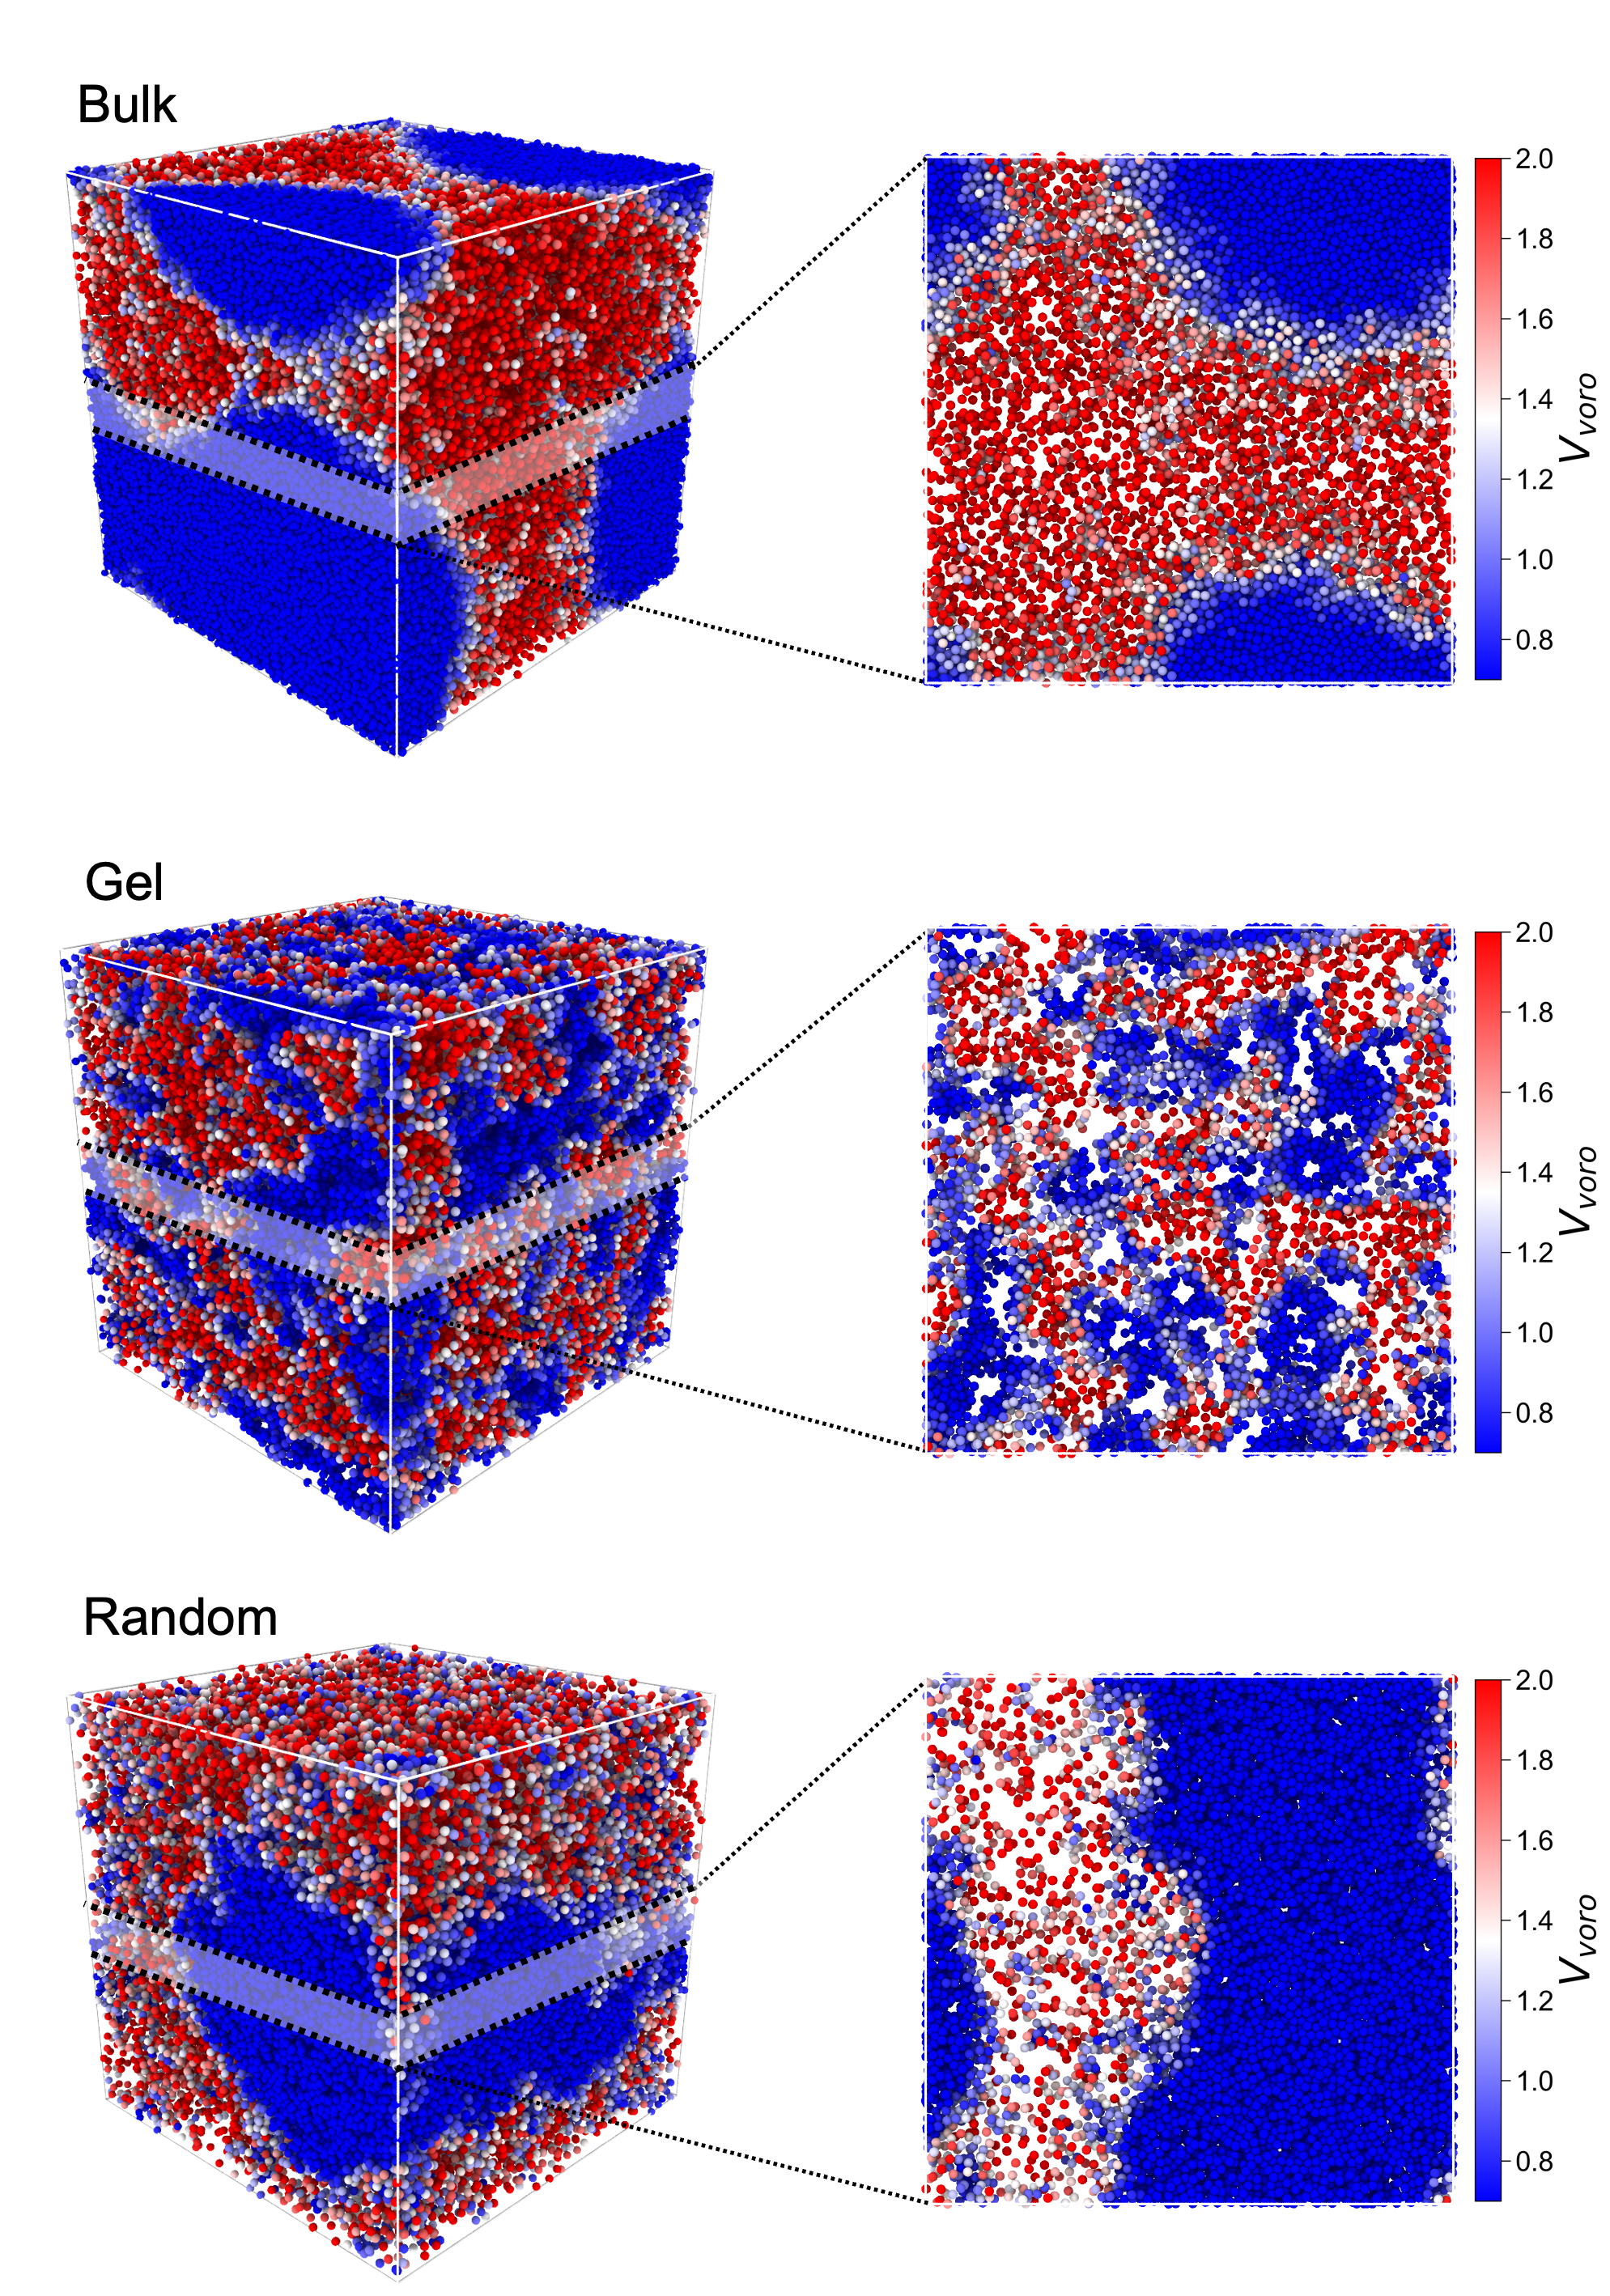
\includegraphics[width=0.9\linewidth]{chapters/activeConfinement/figsActiveConfinement/fig3D_snapshots.png}
	\caption[MIPS in the bulk, gel and pinning systems]{(\textit{Left}) 3D Snapshots of the three systems at $\pecl = 100$, particles are coloured by their Voronoi volumes ($V_{\textrm{voro}}$), obstacles are not rendered. (\textit{Right}) A slice through each system (depth $4\sigma$).}
	\label{fig:fig3D_snapshots}
\end{figure*}


From the results presented in the previous section it is clear that the different confinement types cause significant and varying perturbations to the dynamics of active systems at low $\pecl$. What remains unclear, is the mechanism through which active particles overcome localisation due to the environment, and what behaviour these particles exhibit when mobile at higher Péclet numbers, particularly in the regime of motility induced phase separation (MIPS). 
Compared to the lengthscale of MIPS, we know that the complex environment restricts the active particles to motion over shorter lengthscales; from the chord length measurements, the confining lengthscale is $6.62\sigma$ in the gel and $3.24\sigma$ in the case of random pinning. 
 
We use the individual particle Voronoi volumes ($V_{\textrm{voro}}$) as a measure of the local density to provide insight into the relationship between self-propulsion and complex environments. Fig. \ref{fig:fig3D_snapshots} displays representative snapshots of the bulk, gel network and random pinning systems in the steady-state at high activity ($\pecl = 100$), alongside a slice through each system. In the bulk system (top panel) the particles have undergone motility-induced phase separation. Within the large dense region  particles (coloured dark blue for $V_{\textrm{voro}} \leq 0.8$ in Fig. \ref{fig:fig3D_snapshots}) are clustering due to their persistent motion and are surrounded by a gas of active particles at a lower density.

Fig. \ref{fig:fig3D_snapshots} (middle panel) displays the behaviour of active spheres in gels at high $\pecl$. The structure of the gel is highly complex, featuring extreme variations in surface curvature and channel width. It is clear that this has a strong impact on the dynamics, with a distinct pattern emerging which is clearly dependant on the gel structure. In particular MIPS form a bicontinuous structure, with some pores being filled by the slow/dense phase and others by the fast/less dense phase. 



The influence of the random pinning (bottom panel) on the active particle dynamics at high $\pecl$ is distinct from that of the bulk and gel systems. Here, the particles phase separate into a large cylindrical droplet somewhat akin to the bulk system. However, this droplet has random pins frozen throughout its structure holding the dense phase in space. Furthermore, the presence of the pins brings about an unexpected result: the arrangement of the pins pre-defines the location in which the dense MIPS phase will form. The structure of the MIPS is pinned by the disordered, with independent runs always exhibiting the same demixing pattern. 

\begin{figure}
	\centering
	\includegraphics[width=\linewidth]{chapters/activeConfinement/figsActiveConfinement/figHeatmaps.png}
	\caption[Spacial distribution of $\langle V_{\textrm{voro}} \rangle$ and $\langle \Delta r \rangle$ of ABP in the gel and random pinning systems.]{\textbf{a} Probability density of the Voronoi volumes ($V_{\textrm{voro}}$) in a slice of thickness $\sigma$ in both the gel network (left), and random pinning systems (right). Colours are given by $V_{\textrm{voro}}$, obstacle particles are rendered as white circles.  \textbf{b} Probability density of single particle displacements ($\Delta r$) in the same samples as in (a). Colours are given by $\Delta r$ which are measured over $\Delta t = 6 \tau_R$. All systems are at $\rho=0.87$ and $\pecl=100$}
	\label{fig:heatmaps}
\end{figure}

The three-dimensional snapshots in Fig. \ref{fig:fig3D_snapshots} provide a good indication of the phase behaviour of these systems. However, they do not contain any information on the stability of the dense phase. Therefore, in Fig. \ref{fig:heatmaps}a we plot the average voronoi volume $<V_{\textrm{voro}}>$ as a function of space in both the gel network and random pinning systems. These plots give information regarding the way in which each system phase separates. For the gel, the inclusion of the gel network into the space does not allow for the formation of a single dense droplet as seen in bulk systems experiencing MIPS. Instead, the structure of the gel determines the locations in which the system will phase separate. Given the random nature of the gel, there are sections where the pores are more constricted, have tighter curvature or are less connected; these are the locations that will trap active particles. The spacial distribution of $<V_{\textrm{voro}}>$ in the random pinning system tells an alternate story. Active particles in this system at sufficient $\pecl$ will form a large droplet around a subset of pinned particles. The pins in this droplet keep it stable over long time periods in a steady state where particles are exchanged between the droplet and the surrounding active particle gas.

 The Voronoi volumes give information into the phase separation of these systems but not into the transport dynamics of the individual particles in this environment. Some insight into this aspect can be gained by looking at the average single particle displacements $<\Delta r>$ for the same system. The distributions of $<\Delta r>$ are plotted in Fig. \ref{fig:heatmaps}b for displacements over the time period $t=6\tau_R$, which is a time period of the order of $\tau_{\alpha}$ in the passive bulk system at this density. For the gel system, these displacements are largely uniform in the wider channels. Close to the surfaces of the gel, the displacements are significantly less, indicating shorter movements along the surface. Furthermore, there are several locations where particles become  localised with displacements less than the particle diameter. These are all located in regions of high surface curvature.
 
 
 For displacements in the random system, there are four identifiable types of behaviour. The first is the group of localised particles. These are particles that have become trapped between the pins and other particles in the dense phase and are recognisable as the dark spots dispersed through the dense phase. These are surrounded by the second regime, particles that are not localised but remain trapped within the dense phase and are moving very slowly ($\Delta r < \sigma$). Beyond this is the regime of displacement of particles in the interface, where particles are undertaking mid-range displacements. Finally, outside of the dense phase is the active gas where particles are completing relatively uniform displacements.
 
\begin{figure*}
	\centering
	\includegraphics[width=\linewidth]{chapters/activeConfinement/figsActiveConfinement/figVoro_PDF.pdf}
	\caption[Distribution of Voronoi volumes in the three systems]{Probability density of the Voronoi volumes ($V_{\textrm{voro}}$), for the bulk, porous network, and random pinning systems respectively. All systems are at $\rho=0.87$, and various $\pecl$ (see figure legend).}
	\label{fig:figVORO_histograms}
\end{figure*}

%\subsection{Density fluctuations as a function of $\pecl$}
\textit{Density fluctuations as a function of $\pecl$ ---} So far we have seen examples of how these systems phase separate at $\pecl \approx 100$, now we will look at how the local density fluctuates in these systems for different $\pecl$. The probability density of the Voronoi volumes for each system are determined via kernel density estimation are shown in Fig. \ref{fig:figVORO_histograms} for various $\pecl$. In the absence of activity (ie. $\pecl=0$), all systems feature an approximate Gaussian distribution.
%For the passive particles in the gel system (Fig. \ref{fig:figVORO_histograms}-gel), small peaks outside of the distribution belong to a small population of particles becoming trapped in particularly constricted regions of the gel.
Common to all the environments is the fact that the addition of activity produces a shift in the peak towards smaller volumes and a broadening of the tail of the  distribution towards larger volumes. In the bulk system (Fig. \ref{fig:figVORO_histograms}-bulk) the distributions feature a non-monotonic trend in the spread. First increasing as a function of $\pecl$ up to a maximum at $\pecl = 60$, before decreasing. This is the first sign of re-entrant MIPS behaviour, which will be the focus of Section~\ref{section:Re-entrant dynamics}.
For the gel network (Fig. \ref{fig:figVORO_histograms}-gel) and the random pins (Fig. \ref{fig:figVORO_histograms}-random), this broadening is monotonic, with the gel network covering a wider range of volumes. However, for the random pins and the bulk systems we observe the emergence of twin-peaked distributions at higher activity as a result of phase separation. For both the gel and the random pins, the influence of the complex environment manifests into a splitting of the active particles into more than one population, with some proportion of active particles aggregating or becoming localised through interaction with the environment.

The persistent motion of active particles drives symmetry breaking, this causes them to aggregate at surfaces and walls. In these systems the surfaces could be the edge of a MIPS dense phase, the surface of the gel network, or a dense cluster of pins. These surfaces will collect active particles. To determine how the environment structure affects the collection of particles at surfaces, we count the number of particles located in locally dense regions $N_D$, defined for particles where $V_{\textrm{voro}} < 0.8$. In Fig. \ref{fig:figLocallyDense} we plot the fraction of localised particles $N_{D}/N$ as a function of $\pecl$.


\begin{figure}
	\centering
	\includegraphics[width=0.7\linewidth]{chapters/activeConfinement/figsActiveConfinement/figLocalised.png}
	\caption[Fraction of locally dense particles in the three systems]{The fraction of locally dense particles $N_D / N$.  Particles are considered locally dense if $V_{\textrm{voro}} < 0.8$.}
	\label{fig:figLocallyDense}
\end{figure}

%\subsection{Active transport in complex environments}
\textit{Active transport in complex environments ---}
We have seen so far that with a progressive increase in $\pecl$, all three systems undergo dramatic changes in terms of local density. We have also seen that at high $\pecl$ the average single particle displacements reveal information as to the interaction between the active particles and their environment. As with the Voronoi volumes, we plot the probability densities of active particles in the three systems for various $\pecl$, this time for single particle displacements (Fig \ref{fig:figDR_VORO_corelation}a). At first glance, it is clear that for all systems the particles complete larger displacements as $\pecl$ is increased. Moreover, we see that these distributions are highly featured and reveal a great deal of information as to the behaviour and interactions of the active particles. 

 \begin{figure*}
	\centering
	\includegraphics[width=\linewidth]{chapters/activeConfinement/figsActiveConfinement/figCorrelation.png}
	\caption[Distribution of particle displacements and correlation with Voronoi volumes]{\textbf{a} Probability density of the particle displacements ($\Delta r$), for the bulk, porous network, and random pinning systems respectively. All systems are at $\rho=0.87$, and various $\pecl$ (see figure legend). \textbf{b} Correlation of the Voronoi volumes and the single particle displacements of motile particles in the gel network, random pins and the bulk system. All systems are at a density of $\rho = 0.87$, and plotted for $\pecl = $ 0, 20, and 100. Black lines contain 90\% of data. Colours show contour levels below which the indicated percentage of the data will lie beneath.}
	\label{fig:figDR_VORO_corelation}
\end{figure*}

In the bulk system (Fig. \ref{fig:figDR_VORO_corelation}a-bulk), the $\Delta r$ distribution is a single peaked at $\pecl$=0. As $\pecl$ increases, this distribution shifts to higher displacements and we observe the growth of a second peak; indicating the presence of MIPS in the system. With a further increase of $\pecl$ there is a continuous transition between the relative heights of the peaks as the fraction of particles in the dense phase grows. This is corroborated by the growth of locally dense particles over this range of $\pecl$ observed previously in Fig. \ref{fig:figLocallyDense}. 



The displacements for the gel network and the random pins are plotted in Fig. \ref{fig:figDR_VORO_corelation}a-gel and Fig. \ref{fig:figDR_VORO_corelation}a-random respectively. The distributions of both of these systems show the splitting of a single population into two or more populations with the progressive increase of $\pecl$. The first of these is the emergent peak at very small displacements $\Delta r / \sigma \sim 10^{-1}$. These particles are moving only a small fraction of their diameter and have become localised as a result of the interplay between their activity and the environment.
Interestingly, both systems in complex environments (Fig. \ref{fig:figDR_VORO_corelation}a-gel/random) feature a strong peak at $\Delta r / \sigma = 1$, with some smaller features at subsequent integer displacements. Through cross examination of the average displacements in Fig. \ref{fig:heatmaps}, these displacements are located along the surfaces of the gel network and in small pockets of lower density in the dense phase of the pinning system. The location of these displacements makes it clear that these are a result of particle re-arrangements at the obstacle interface, and in dense particle clusters. 
For the gel network (Fig. \ref{fig:figDR_VORO_corelation}a-gel) at $Pe > 0$, the remaining particles are in a single large population, moving comparable distances to particles in the bulk system. Whereas, in the random pins (Fig. \ref{fig:figDR_VORO_corelation}a-random), at $\pecl \geq 40$ there is a splitting of larger displacements across two length scales, one at the interface and the second in the active gas.


Thus far we have been primarily looking at two observables $V_{\textrm{voro}}$ and $\Delta r$, both of which tell part of the story. These two observables can be correlated to complete this picture, the result of which is plotted in Fig. \ref{fig:figDR_VORO_corelation}b. This plot shows a series of contours stacked logarithmically, each layer denotes the level at which a percentage of the data lies below. These plots provide some insight into the population splitting phenomena we have seen so far. We see that the combination of confinement and activity create a subpopulation of particles that are arrested and have very little free space,  a feature not found in the bulk system. Interestingly, this arrested group is relatively larger in the random pinning system. For the systems at high $\pecl$ in Fig. \ref{fig:figDR_VORO_corelation}b, the particles that have $V_{\textrm{voro}} < 0.8$ and are in some form belonging to dense clusters, the particles still cover a wide range of displacements. 
This is likely a combination of two phenomena, the first is particles that have been localised over a long time frame. These are particles that are not moving and have very little free space. The other case is particles which have been mobile but are now located in a dense cluster or at the object interface. 


\subsection{Local structure}
\label{section:Local structure}
In Fig. \ref{fig:figTCC} we study the local structure of the active fluid (excluding the obstacles) via the topological cluster classification (TCC) method. The TCC can identify local environments that are energy minima of clusters of size $m$ of an equilibrium reference system (here, the Lennard--Jones model). We consider how the population of the different environments ($N_c / N$) changes as a function of activity as well as the influence of the local environment, where $N_c$ is the number of particles participating in a particular cluster. To identify the cluster population, a bond network is identified with a modified Voronoi decomposition, where the Voronoi parameter is set $f_c=0.82$ \cite{malins2013}. In order to identify the clusters, we include the immobilised particles in the bond network when performing the TCC analysis. However, for $N_c$ (and $N$), we only consider active particles.

\begin{figure*}
	\centering
	\includegraphics[width=\linewidth]{chapters/activeConfinement/figsActiveConfinement/figTCC_labelled.png}
	\caption[Local structure in the three systems]{Mean cluster population $N_c / N$ as a function of $\pecl$ in the  bulk, gel and random systems at $\rho=0.87$. Colours correspond to the clusters depicted in the legend.}
	\label{fig:figTCC}
\end{figure*}


Fig. \ref{fig:figTCC} shows a common trend between the bulk, gel and random environments: the equilibrium local structure population is disrupted by increasing $\pecl$. Confined environments both show cluster populations that are lower compared to the bulk case. The random environment, where the position of the obstacles is taken from equilibrium configurations, at $\pecl=0$ has the same population numbers as the bulk case, but as soon as activity is switched on all cluster populations fall more abruptly compared to the bulk case. The first rapid decrease in local structure at $\pecl\simeq 30$ coincides with the formation of MIPS. Differently from the gel and random case, the bulk experiences another big drop in local structure population for $\pecl\simeq 140$. As we will see in the next Section, this drop corresponds to a reentrant MIPS behaviour that is observed only in the bulk case.

 


\subsection{Reentrant mixing}
\label{section:Re-entrant dynamics}

In addition to the phase behaviour discussed thus far, there is one final relevant phase for suspensions of active spheres: At very high $\pecl$, active spheres will transition from a MIPS dense phase into a homogeneous active fluid. A similar behaviour has been observed previously in ref.~\cite{bialke2013,stenhammar2014,su2022} in bulk systems.
We confirm these observations in the bulk case. The presence of the transition is apparent in the probability density of $V_{\textrm{voro}}$ in the bulk system (Fig. \ref{fig:re-entant}a). These distributions show two populations at  intermediate $\pecl$, but a single population at $\pecl=0$ and at $\pecl > 120$. Looking at the correlation of $V_{\textrm{voro}}$ with $\Delta r$ confirms the single reentrant phase at high $\pecl$ (Fig. \ref{fig:re-entant}b). 
\begin{figure*}
	\centering
	\includegraphics[width=\linewidth]{chapters/activeConfinement/figsActiveConfinement/figRe-entrant.png}
	\caption[Reentrant phase separation]{\textbf{a} Probability density of the Voronoi volumes in the bulk system at various $\pecl$. As $\pecl$ increases the distributions show first one, then two populations, and then a re-entrant single phase at high $\pecl$. \textbf{b} Correlation of $V_{\textrm{voro}}$ and $\Delta r$ in the bulk system at $\pecl=160$ shows a single population. \textbf{c} Variance of the distribution of Voronoi volumes in the porous network, random pinning and the bulk systems as a function of $\pecl$, all at density $\rho = 0.87$.}
	\label{fig:re-entant}
\end{figure*}
To study the reentrant phase behaviour in systems with quenched disorder in Fig. \ref{fig:re-entant}c we plot the variance of the probability density of $V_{\textrm{voro}}$ as a function of $\pecl$: non monotonic behaviour in this quantity signals a reentrant phase.
Looking at this data we can see that for the bulk and random systems, as $\pecl$ increases, the variance also increases up to a maximum; beyond which it decays to an intermediate value. The peak corresponds to the state where there is a roughly equal fraction of particles in the dilute and dense phases $N_D / N \approx 1/2$. We plot the same for the systems with confinement in Fig. \ref{fig:re-entant}c. Notably, the random pinning system also undergoes a transition to a reentrant fluid. However this transition is delayed relative to the bulk, indicating that the presence of the pins works to stabilise the MIPS phase at high $\pecl$.
For the gel system we do not observe the reentrant behaviour within the considered range of $\pecl$.


\section{Conclusion}
\label{section:conclusion}
Suspensions of active Brownian spheres show a rich collection of dynamical behaviour, and our goal was to explore whether that collective behaviour is
present in constricted random environments at high densities. To do this, we prepared quenched disordered configurations with different static properties: randomly pinning particles from equilibrium bulk configurations and from a porous gel structure. Both random environments are constructed to have the same free volume available to the mobile particles, thus allowing a direct comparison of the effects of the static lengthscale of the confinement on the behaviour of active particles.

We first explored the phase behaviour at low $\pecl$ revealing how pinning suppresses the crystallisation of the fluid at high densities. The relaxation time of the particles is slowed down by the obstacles (more for the random case compared to the gel case) and the dynamics become more dynamically heterogeneous, as confirmed by the study of the overlap function and four-point susceptibility.
At intermediate $\pecl$ the bulk system displays MIPS, where the systems form domains of dense/slow regions and low density/fast regions. Perhaps surprisingly, we find that the obstacles not only do not suppress MIPS formation, but actually act to stabilise them.
Random obstacles display a very similar phase-separation pattern as the bulk case, however the domains do not appear homogeneously in the system, but are always formed from the same regions of the sample. The mechanism for the nucleation of MIPS from random obstacles is still unknown, and should be addressed in future studies.
In the case of the gel, the MIPS domains change completely, and form a bicontinuous network where the active and inactive regions occupy different pores of the structure.

Finally we considered how local structure is perturbed by the activity, and revealed that reentrant mixing behaviour is suppressed (or moved to higher $\pecl$) by the random environments. In particular the gel environment seems to be the most effective in stabilising the density and activity fluctuations. In this case, we attributed this behaviour to the absorption at the rough walls, where the persistent motion of active particles creates localised and highly dense regions, which in turn frees space inside the pores that increase particle transport in the system.
We believe that these results could be important for better understanding transport in biological environments and for guiding future studies of active matter particles in random media.



%\section*{Appendix}
%
%\subsection*{Overlap}
%
%
%
%The overlap function $Q(t)$ compares a particle configuration with itself at a later time. An important feature of this measure of similarity is that it is not particle specific, it matters not whether it is the same particle occupying that space, only that there is a particle there. With this in mind, it is clear why the bulk system (Fig. \ref{fig:Chi4}a) behaves as it does. In this system, there are no fixed obstacles, and thus there are no points at which a cluster of particles could be anchored. Therefore, even in a system with MIPS present the centre of mass of a dense cluster remains diffusive and thus $Q(t)$ decays to a small value. $Q(t)$ does not decay to $0$ in this case in the bulk due to the relatively high density, as there will always be some degree of overlap.
%
%For active particles in the other two systems, there is clear evidence of the interplay between the self-propulsion and the complex environment. Both systems converge to an overlap value, higher than that of the bulk system. This is a product of the fixed geometry of the obstacles. Although the obstacle particles are not considered, there will be regions in structure that will be more likely to trap active particles, and even though particles are mobile, there is a high probability that there will be some particles in these regions. Interestingly, the gel and the random pins approach their convergent overlaps from different directions as $\pecl$ increases. For the gel system (Fig. \ref{fig:Chi4} b), the overlap value $Q(t)$ increases with $\pecl$ at longer times, while decreasing with an increased rate at shorter times. The increased rate on short timescales is explained by the increased propulsion velocity promoting a quicker re-configuration of the active particle populations. However, this increase in $\pecl$ has the added effect of increasing the likely hood of a particle becoming trapped against the walls of the gel network, this is supported by the increase in the localised fraction  $N_{\textrm{loc}}/N$ with $\pecl$ in Fig. \ref{fig:figLocallyDense}.
%
%Like in the bulk and the gel network, the overlap of the random system also decays at an increasing rate as $\pecl$ increases at short times (Fig. \ref{fig:Chi4} c). In the absence of activity, the random system particles have a very slow decay in $Q(t)$. This is a result of the pinned particles dramatically slowing down the dynamics of passive particles, this also seen in the $\alpha$-relaxation time in Fig. \ref{fig:TauAlpha}, where $\tau_{\alpha}$ was measured to be of the order $10^4$ larger than that of the bulk or gel systems. Unlike in the gel system, $Q(t)$ for the random pinning approaches its convergent value from above. This is likely due to the arrangement of the obstacles in the random pinning system, since the pinned particles are dispersed through the entire space, the active particles have a higher chance of becoming trapped. The random system converges to have higher overlap value than the gel, this is due to the larger fraction of particles in the becoming localised in the random system than in the gel.
%
%\begin{figure*}
%	\centering
%	\includegraphics[width=\linewidth]{figOverlap.png}
%	\caption{(\textit{a,b,c}): The overlap $Q(t)$ for particles in the bulk, gel, and random systems at $\rho = 0.87$ for various Pe (see legend).}
%	\label{fig:Chi4}
%\end{figure*}
%
%\begin{figure}
%	\centering
%	\includegraphics[width=\linewidth]{figVoroVariance_FiniteSize.png}
%	\caption{Variance of the distribution of Voronoi volumes in the porous network, random pinning and the bulk system, all at density $\rho = 0.87$.}
%	\label{fig:figVoroVariance}
%\end{figure}
%
